\documentclass[11pt,a4paper,titlepage,onecolumn]{report}

% Corrigir margens e paragrafos
\usepackage[hmarginratio=1:1]{geometry}
\usepackage{parskip}
\usepackage{mathtools}
\usepackage{amsfonts}
\usepackage[titletoc]{appendix}
\usepackage{float}
\usepackage{pdflscape}

% Definir linguagem portuguesa
\usepackage[utf8]{inputenc}
\usepackage[T1]{fontenc}
\usepackage[portuguese]{babel}

\setlength{\textheight}{21cm}
\setlength{\voffset}{-0.5cm}

% Incluir packages de cores
\usepackage{graphicx}
\usepackage{color}
\usepackage{xcolor}

\usepackage{listings}

\usepackage{indentfirst}
\parindent=18pt

\usepackage{chngcntr}
\linespread{1.3}
\usepackage[T1]{fontenc}
\usepackage{titlesec, blindtext, color}
\definecolor{gray75}{gray}{0.75}
\newcommand{\hsp}{\hspace{20pt}}
\titleformat{\chapter}[hang]{\Large\bfseries}{\chaptername \ \thechapter\hsp\textcolor{gray75}{|}\hsp}{0pt}{\LARGE\bfseries}

\lstset{
	language=C,
	tabsize=2,
	basicstyle=\ttfamily,
	breaklines=true,
	keywordstyle=\color{blue}\ttfamily,
	stringstyle=\color{red}\ttfamily,
	commentstyle=\color{green}\ttfamily,
	morecomment=[l][\color{magenta}]{\#}
}

\begin{document}
	
	\begin{titlepage}
	% Desactivar a contagem das páginas durante o título
	\pagenumbering{gobble}
	
	\begin{center}
		
		% Logo
		
\includegraphics[trim = 4cm 4cm 4cm 4cm, keepaspectratio=true, height=2.5cm]{IST_LOGO.pdf}~\\[0.5cm]
		
		% Instituto, Cadeira
		\textsc{\LARGE Instituto Superior Técnico\\[0.5cm]
		               MEEC\\[0.5cm]
		               2º Semestre 2014/2015\\[2cm]
		               \huge \bfseries Arquitecturas Avançadas de Computadores}\\[3cm]
		
		
		% Título
		\huge \bfseries Projecto 3\\[0.5cm]
		\vfill
		\large
		
		% Subtítulo
		Paralelização e aceleração de um programa em CUDA \\[0.5cm]
		\vfill
		
		Trabalho realizado por:\\
		\begin{tabular}{l r}
			João Baúto & Nº 72856\\
			João Severino &  Nº 73608\\
		\end{tabular}
		\vfill
		% Bottom of the page
		{\large 
			Professor: Leonel Sousa
			}
	\end{center}
	
	% Reactivar a contagem das páginas
	\cleardoublepage
	\setcounter{page}{1}
	\pagenumbering{arabic}
\end{titlepage}

	\renewcommand{\contentsname}{Índice}
	\tableofcontents
	\addtocontents{toc}{\hfill\textbf{Página}\par}
	\chapter{Introdução}
O objectivo deste terceiro trabalho de laboratório é a aceleração de um algoritmo de \textit{smoothing} utilizando as propriedades de computação paralela em GPUs.

Para tal recorreu-se à plataforma CUDA\texttrademark  que tira proveito das unidades de processamento gráfico (GPUs) da NVIDIA\texttrademark.

Procura-se tirar proveito da arquitectura dos GPUs para maximizar o desempenho de um algoritmo de \textit{smoothing} recorrendo ao Paralelismo de Dados.

\section{Algoritmo}

O algoritmo de \textit{smoothing} é um algoritmo bastante utilizado no processamento de imagem bem como análise estatística com o objectivo de criar uma função aproximada dos dados de entrada mantendo pontos importantes nos dados enquanto que reduz qualquer tipo de ruído associado aos dados. 

Para modelar os dados o algoritmo observa um ponto individual bem como os imediatamente adjacentes e caso o ponto a observar seja maior em valor que os seus adjacentes é suavizado diminuindo o seu valor. Se o valor for menor que os seus adjacentes é entre elevado o seu valor em relação à sua volta. Isto assume que estas elevações bruscas de valores deve-se a ruído no sinal.

O algoritmo que pretendemos paralelizar consiste em:
\[ \hat{y}_i=\frac{\sum_{k=0}^{N-1} K_{b}(x_i,x_k)y_k}{\sum_{k=0}^{N-1} K_{b}(x_i,x_k)} \]
com
\[ K_b(x,x_k)=exp\left ( -\frac{\left ( x-x_k \right )^2}{2b^2} \right ) \]
onde
\begin{description}
	\item[x] \hfill \\
	Domínio do sinal a ser filtrado
	\item[y] \hfill \\
	Sinal observado e que contém ruído e do qual pretendemos obter a versão sem ruído
	\item[$\hat{y}$] \hfill \\
	Sinal obtido pela passagem do sinal y pela função de \textit{smoothing}
	\item[b] \hfill \\
	Parâmetro de \textit{smoothing}, no nosso caso foi utilizado o valor 4 para este parâmetro
\end{description}
	\chapter{Código C}
Para servir como ponto de partida e de comparação com os resultados obtidos quando utilizado o \textbf{GPU} foi desenvolvido este código em C com base no exemplo dado no enunciado.\\

\lstinputlisting[frame=single]{main.c}

Este código executa o algoritmo e calcula e imprime para o terminal o tempo que demora a fazê-lo, e em seguida imprime os dados para um ficheiro de saída.

Um gráfico exemplificativo do funcionamento deste código apresenta-se a seguir, o código foi executado na máquina Diana que nos foi disponibilizada e onde demorou um tempo mediano de 3,862388
segundos.\\

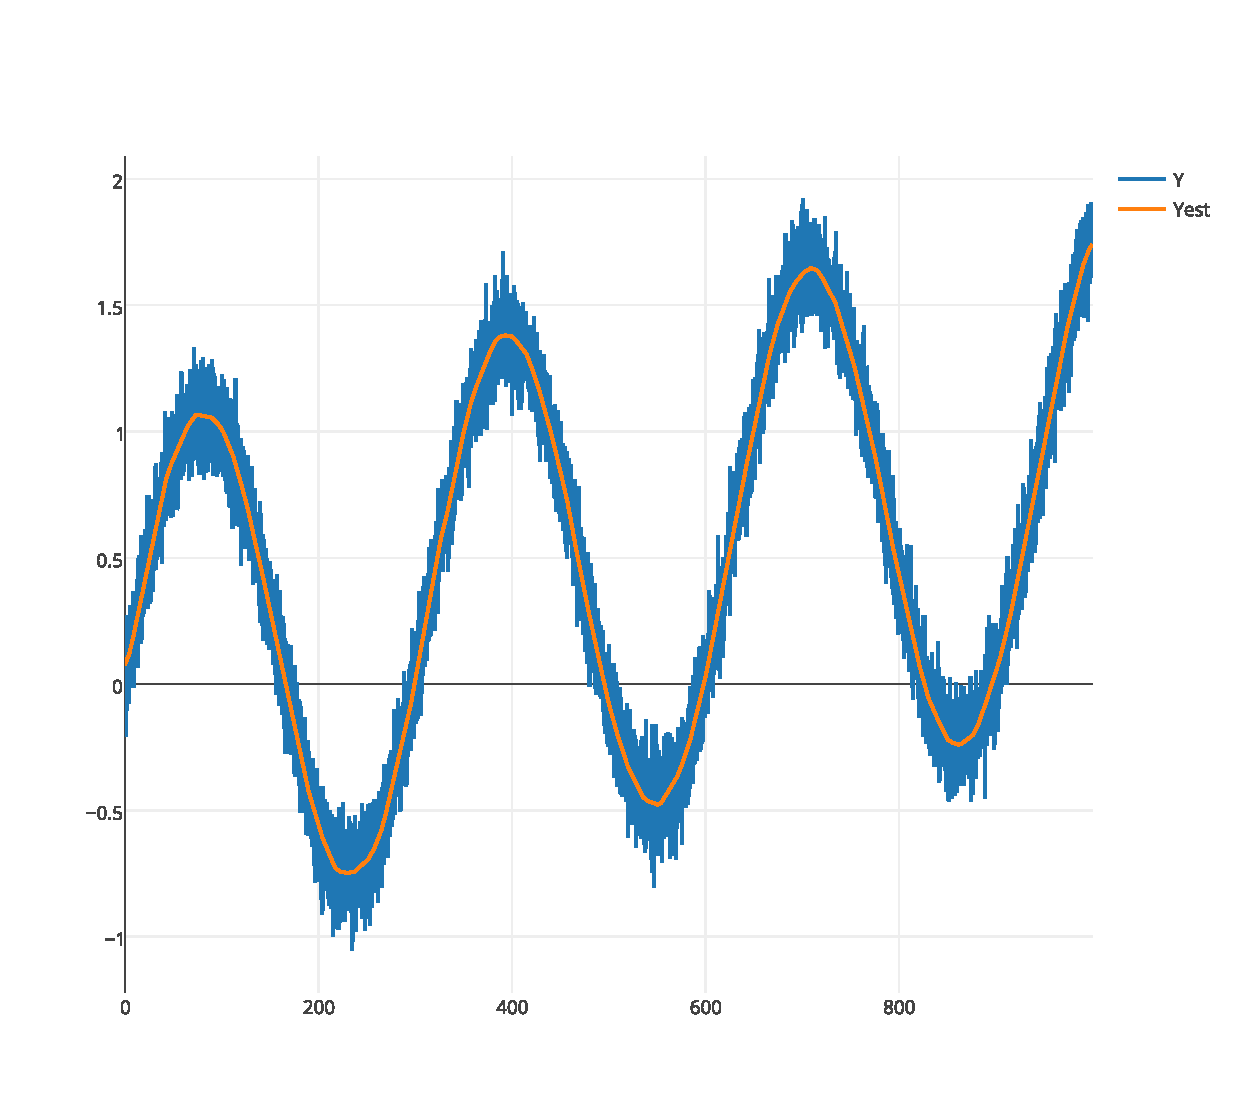
\includegraphics[width=\textwidth]{output}
	\chapter{Código para o GPU}
Para optimizar a aceleração do algoritmo de ``smoothing'' no \textbf{GPU} começámos por analisar as diversas chamadas ao \textbf{GPU} e concluímos que as que consomem mais tempo são a inicialização e as transferências de dados entre o \textbf{Host} e o \textbf{GPU} e entre o \textbf{GPU} e o \textbf{Host}, sendo que a execução do \textbf{Kernel} em si consome uma porção quase negligenciável.\\

Com estas informações e tendo em conta que as chamadas de inicialização são constantes e não se podem alterar procurámos primeiro otimizar as transferências de dados e só depois otimizar o \textbf{Kernel}.

\section{Transferências de Dados}


\section{Kernel}


	\chapter{Resultados}
\label{chap:res}
Na tabela \ref{tabela} são apresentados os resultados obtidos para o algoritmo de \textit{smoothing}. Foram feitos testes para valores de N até 80000 sendo feita uma descrição detalhada do tempo para cada secção do programa desenvolvido. Nas tabelas \ref{tabela1} e \ref{tabela2} é feita uma previsão dos tempos quer para o CPU quer para o GPU (previsão feita com base nas linhas de tendência dos valores até 80000).

\begin{figure}[H]
	\begin{center}
		\makebox[\textwidth][c]{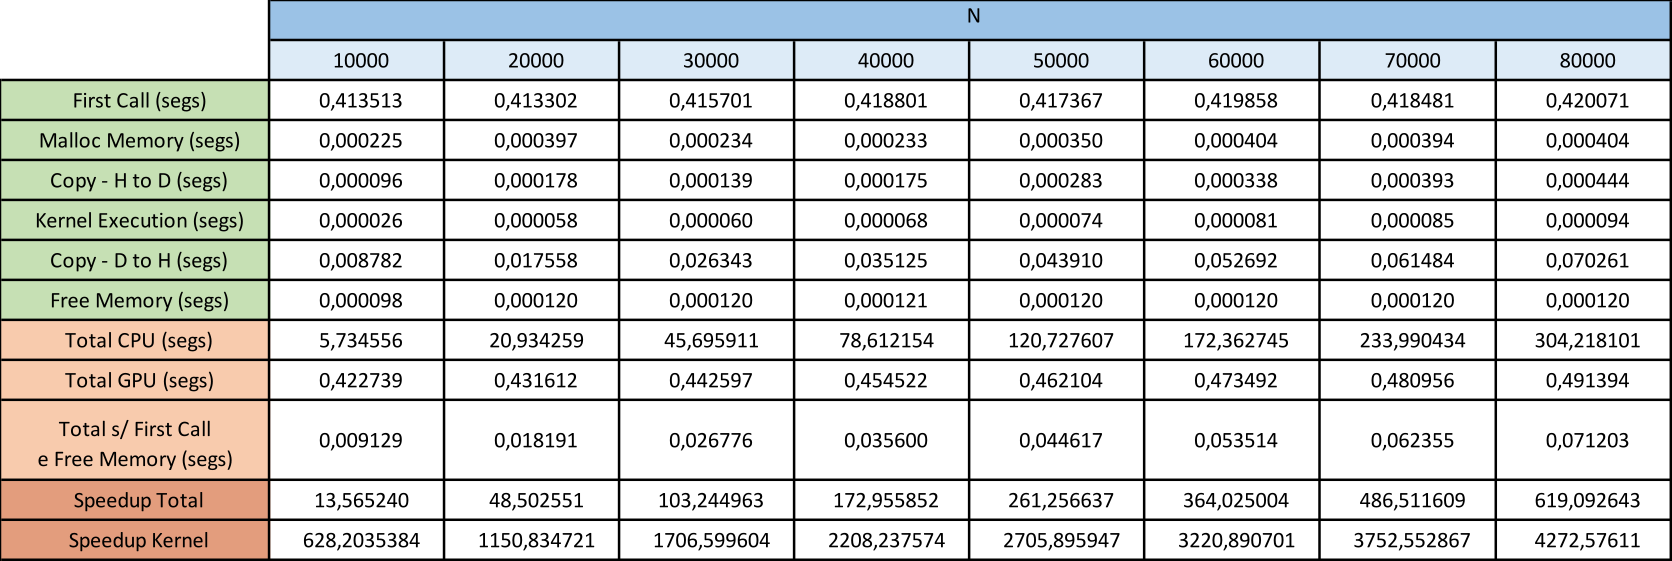
\includegraphics[clip, keepaspectratio=true, scale=3.5]{tabela.png}}
		\caption{Resultados Obtidos.}
		\label{tabela}
	\end{center}
\end{figure}

\begin{figure}[H]
	\begin{center}
		\makebox[\textwidth][c]{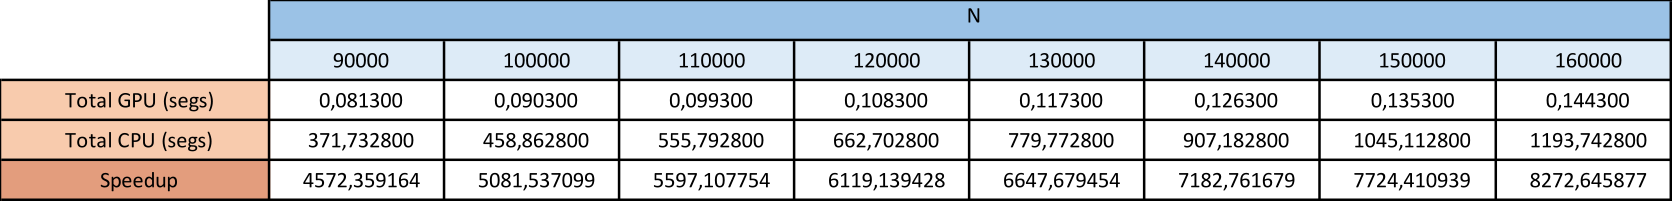
\includegraphics[clip, keepaspectratio=true, scale=3.5]{tabela1.png}}
		\caption{Previsão de Resultados.}
		\label{tabela1}
	\end{center}
\end{figure}

\begin{figure}[H]
	\begin{center}
		\makebox[\textwidth][c]{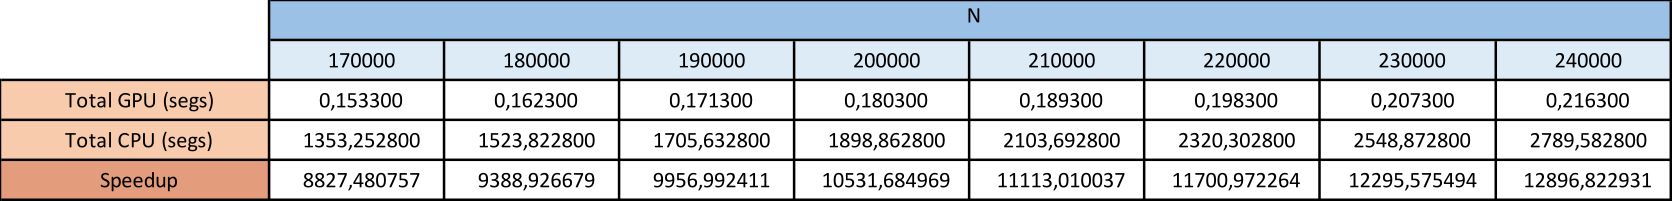
\includegraphics[clip, keepaspectratio=true, scale=3.5]{tabela2.png}}
		\caption{Previsão de Resultados (continuação).}
		\label{tabela2}
	\end{center}
\end{figure}

Com os valores obtidos através de baterias de 30 execuções para cada N foram elaborados os gráficos com o tempo de execução do CPU, do GPU, do Kernel e por fim da relação N - Speedup.

\begin{figure}[H]
	\begin{center}
		\makebox[\textwidth][c]{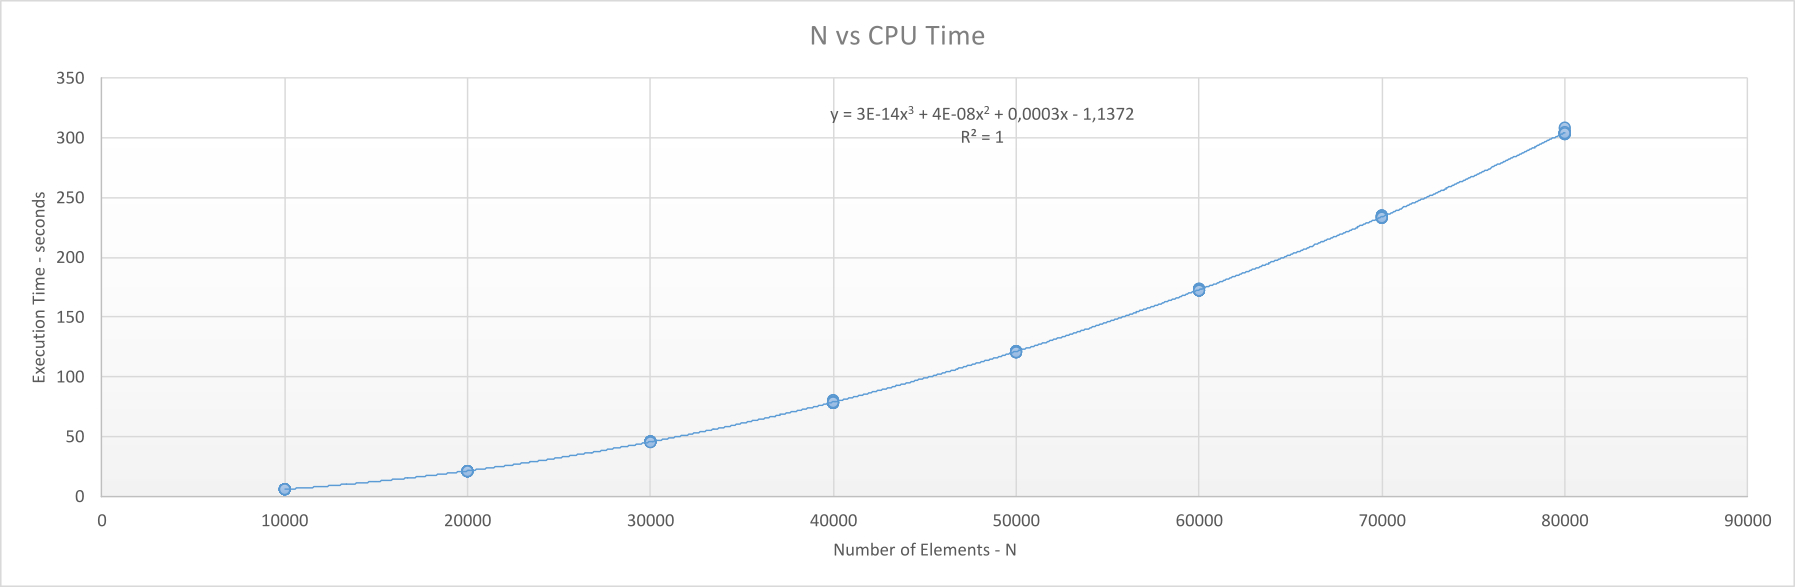
\includegraphics[clip, keepaspectratio=true, scale=2.5]{cpu.png}}
		\caption{Relação N - Tempo de CPU.}
		\label{cpu}
	\end{center}
\end{figure}

\begin{figure}[H]
	\begin{center}
		\makebox[\textwidth][c]{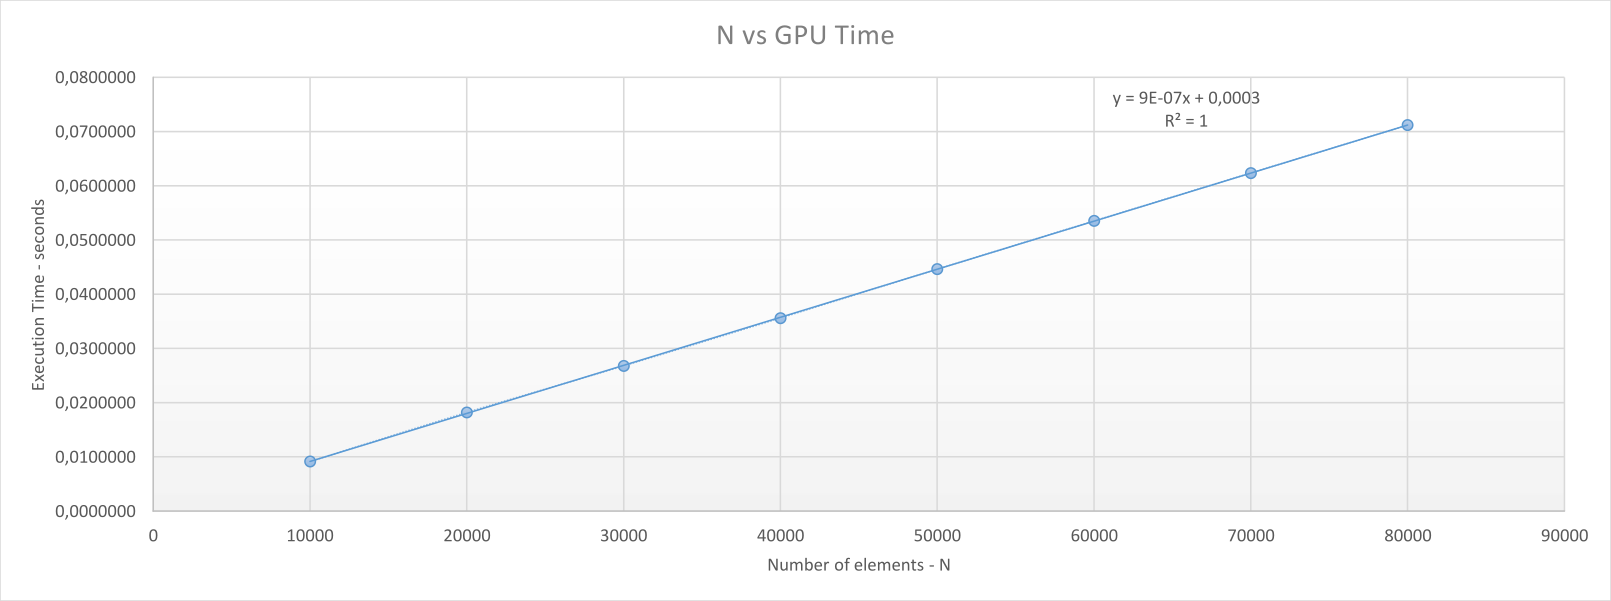
\includegraphics[clip, keepaspectratio=true, scale=2.5]{gpu.png}}
		\caption{Relação N - Tempo de GPU.}
		\label{gpu}
	\end{center}
\end{figure}

\begin{figure}[H]
	\begin{center}
		\makebox[\textwidth][c]{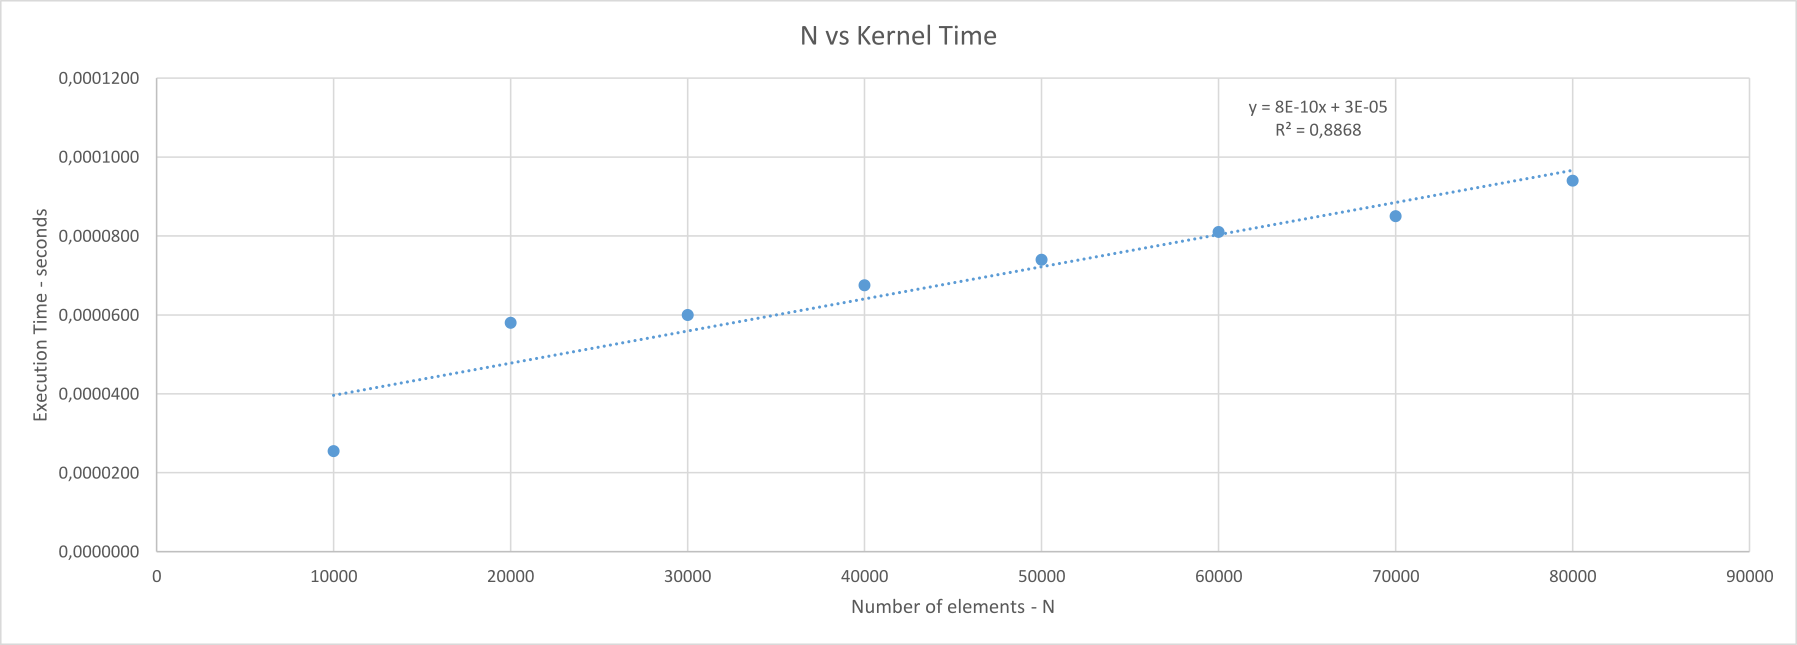
\includegraphics[clip, keepaspectratio=true, scale=2.5]{kernel.png}}
		\caption{Relação N - Tempo de Kernel.}
		\label{kernel}
	\end{center}
\end{figure}

\begin{figure}[H]
	\begin{center}
		\makebox[\textwidth][c]{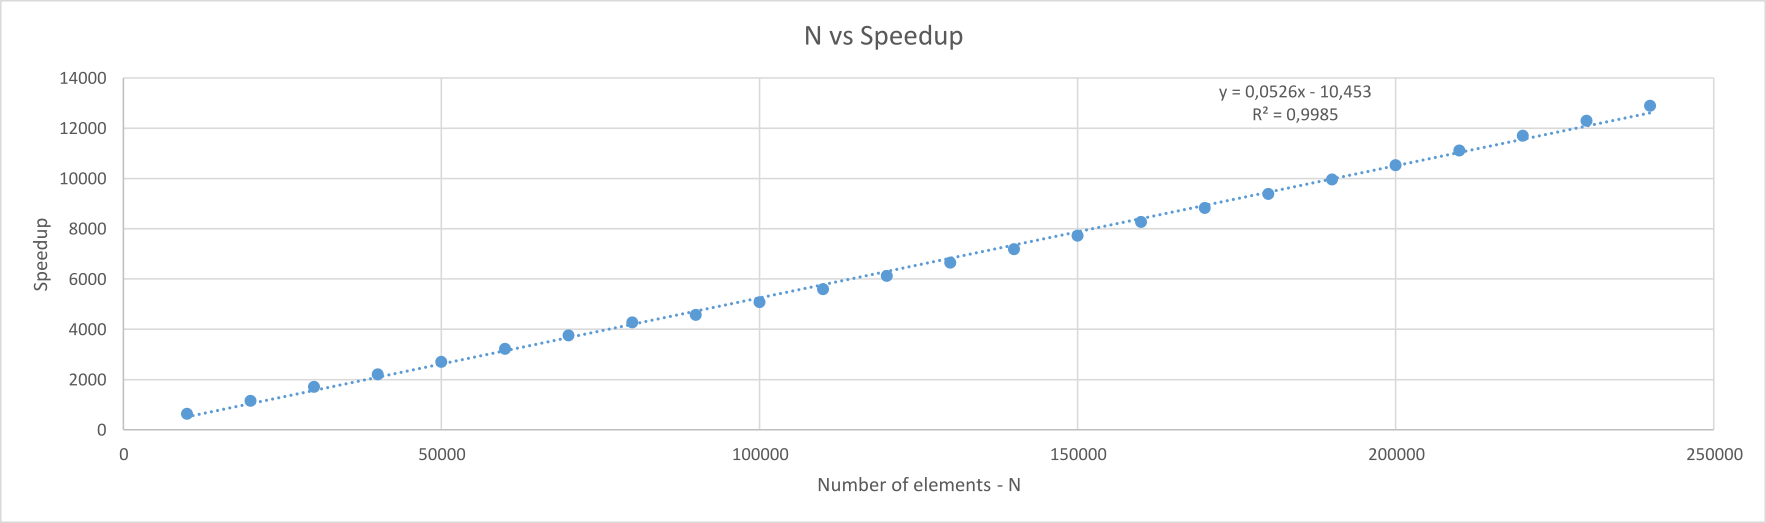
\includegraphics[clip, keepaspectratio=true, scale=2.5]{speedup.png}}
		\caption{Relação N - Speedup.}
		\label{speedup}
	\end{center}
\end{figure}

Por observação dos gráficos \ref{cpu} e \ref{gpu} é óbvio a utilização de \textit{GPUs} para este tipo de algoritmo. No caso do \textit{CPU} para N elevados o tempo de execução começa-se a obter uma função do tipo exponencial ao contrário do \textit{GPU} que mantêm um comportamento linear com crescimento imposto pelo tempo de tranferência de dados do \textit{Device} para o \textit{Host}.

Apesar de não serem apresentados valores de tempo para N inferior a 10000, tal como verificado na demonstração do programa na aula, o \textit{GPU} apresenta valores de Speedup inferior a 0.3 para N igual a 1000 e desta forma para valores de N baixos não se justifica a utilização de \textit{GPU} para este tipo de algoritmo. 

	\chapter{Conclusão}
	\renewcommand{\thechapter}{\Alph{chapter}}
\renewcommand{\thesection}{\Alph{chapter}.\arabic{section}}
\setcounter{chapter}{0}
\chapter{Anexos}
\section{CPU}
\lstinputlisting[frame=single, firstline=125, lastline=141]{kernel.cu}
\newpage

\section{Kernel GPU}
\label{secA:kernel}
\lstinputlisting[frame=single, firstline=12, lastline=30]{kernel.cu}
\newpage

\section{Código final}
\lstinputlisting[frame=single]{kernel.cu}
	
\end{document}